%!TEX root = ../../book_ML.tex
\chapter{Lọc cộng tác lân cận}
% \chapter{Neighborhood-based collaborative filtering}
\label{cha:CF}
 
\section{Giới thiệu}

\index{hệ thống gợi ý -- recommendation system!lọc cộng tác lân cận -- neighborhood-based collaborative filtering}
 
Trong hệ thống gợi ý dựa trên nội dung, chúng ta đã làm quen với một hệ thống
gợi ý sản phẩm đơn giản dựa trên vector đặc trưng của mỗi sản phẩm. Đặc điểm của
các hệ thống này là việc xây dựng mô hình cho mỗi người dùng không phụ thuộc vào
các người dùng khác mà chỉ phụ thuộc vào thông tin sản phẩm. Việc làm này có lợi
thế là tiết kiệm bộ nhớ và thời gian tính toán nhưng có hai nhược điểm cơ bản.
Thứ nhất, việc xây dựng thông tin cho sản phẩm không phải lúc nào cũng thực hiện
được. Thứ hai, khi xây dựng mô hình cho một người dùng, các hệ thống gợi ý theo
nội dung không tận dụng được thông tin đã có từ những người dùng khác. Những
thông tin này thường rất hữu ích vì hành vi mua hàng của người dùng thường được
chia thành một vài nhóm cơ bản. Nếu biết hành vi mua hàng của một vài người dùng
trong nhóm, hệ thống nên có khả năng dự đoán hành vi của những người dùng còn
lại trong nhóm đó.
 
Những nhược điểm này có thể được giải quyết bằng một kỹ thuật có tên là \textit{lọc cộng tác} (collaborative filtering -- CF)~\cite{schafer2007collaborative,
ekstrand2011collaborative}. Trong chương này, chúng ta cùng làm quen với một
phương pháp CF có tên là \textit{lọc cộng tác dựa trên lân cận} (neighborhood-based collaborative filtering -- NBCF). Chương tiếp theo sẽ trình bày về một phương pháp CF khác có tên \textit{lọc cộng tác phân tích ma trận}
(matrix factorization collaborative filtering). Nếu chỉ nói
\textit{lọc cộng tác}, ta gầm hiểu rằng đó là
\textit{lọc cộng tác dựa trên lân cận}.
 
Ý tưởng của NBCF là xác định {mức độ quan tâm} của một người dùng tới một sản
phẩm dựa trên những người dùng có hành vi tương tự. Việc xác định sự tương tự
giữa những người dùng có thể được xác định thông qua {mức độ quan tâm} của họ
tới các sản phẩm khác mà hệ thống đã biết.  Ví dụ, $A$ và $B$ thích phim
``{Cảnh sát hình sự}'', đều đã đánh giá bộ phim này năm sao. Ta đã biết thêm
\textit{A} thích ``{Người phán xử}'', vậy nhiều khả năng \textit{B} cũng
thích bộ phim này.
 
Có hai câu hỏi chính khi xây dựng một hệ thống lọc cộng tác dựa trên lân cận:
\begin{enumerate}
    \item Làm thế nào xác định được {sự tương tự} giữa hai người dùng?
    \item Khi đã xác định được các người dùng có hành vi {gần giống nhau}, làm thế nào dự đoán được {mức độ quan tâm} của một người dùng lên một sản phẩm?
\end{enumerate}
 
Việc xác định mức độ quan tâm của mỗi người dùng tới một sản phẩm dựa trên mức
độ quan tâm của những người dùng tương tự tới sản phẩm đó còn được gọi là
\textit{lọc cộng tác người dùng} (user-user collaborative filtering). Có
một hướng tiếp cận khác thường cho kết quả tốt hơn là \textit{lọc cộng tác
sản phẩm} (item-item collaborative filtering). Trong hướng tiếp cận này, thay vì
xác định độ tương tự giữa các người dùng, hệ thống sẽ xác định độ tương tự
giữa các sản phẩm. Từ đó, hệ thống gợi ý một sản phẩm tương tự những sản phẩm
khác mà người dùng đó có mức độ quan tâm cao.
 
Cấu trúc của chương như sau: Mục~\ref{sec:uu} trình bày lọc cộng tác người
dùng. Mục~\ref{sec:ii} nêu một số hạn chế của phương pháp này và cách khắc phục
bằng lọc cộng tác sản phẩm. Kết quả của hai phương pháp này được trình bày
qua ví dụ trên cơ sở dữ liệu MovieLens 100k trong Mục~\ref{sec:24_python}.
Mục~\ref{sec:24_discuss} thảo luận các ưu nhược điểm của NBCF.
 
 
\section{Lọc cộng tác theo người dùng}
\index{hệ thống gợi ý -- recommendation system!lọc cộng tác người dùng -- user-user collaborative filtering}
\label{sec:uu}
\subsection{Hàm số đo độ tương tự}
Việc quan trọng nhất trong lọc cộng tác người dùng là xác định được
\textit{độ tương tự} ({similarity}) giữa hai người dùng. Giả sử thông tin duy
nhất chúng ta có là ma trận tiện ích $\mathbf{Y}$. Độ tương tự giữa hai người
dùng sẽ được xác định dựa trên các cột tương ứng với họ trong ma trận này.

\index{hàm đo độ tương tự -- similarity function}
Xét ví dụ trong Hình \ref{fig:24_1}. Giả sử có những người dùng từ $u_0$ đến
$u_6$ và các sản phẩm từ $i_0$ đến $i_4$.  Các số trong mỗi ô vuông thể hiện {số
sao} mà mỗi người dùng đã đánh giá sản phẩm với giá trị cao hơn thể hiện {mức
quan tâm} cao hơn. Các dấu hỏi chấm là các giá trị mà hệ thống cần tìm. Đặt {mức
độ tương tự} của hai người dùng $u_i, u_j$ là $\text{sim}(u_i, u_j)$. Có thể
nhận thấy $u_0, u_1$ {thích} $i_0, i_1, i_2$ hơn $i_3, i_4$. Trong khi đó $u_2,
u_3, u_4, u_5, u=_6$ thích $i_3, i_4$ hơn $i_0, i_1, i_2$. Vì vậy, một
\textit{hàm đo độ tương tự} ({similarity function}) tốt cần đảm bảo:
\begin{equation}
\text{sim}(u_0, u_1) > \text{sim}(u_0, u_i), ~\forall i > 1,
\end{equation} 
với giá trị cao hơn ứng với độ giống nhau cao hơn. 

Để xác định {mức độ quan tâm} của $u_0$ lên $i_2$, chúng
ta nên dựa trên {hành vi} của $u_1$ lên sản phẩm này. Vì đã biết $u_1$ {thích} $i_2$, hệ thống có thể gợi ý $i_2$ tới $u_0$.
 
Câu hỏi đặt ra là, hàm đo độ tương tự cần được xây dựng như thế nào? Để đo độ
tương tự giữa hai người dùng, cách thường làm là xây dựng vector đặc trưng cho
mỗi người dùng rồi áp dụng một hàm có khả năng đo độ giống nhau giữa hai vector
đó. Ở đây, việc xây dựng vector đặc trưng khác với việc xây dựng thông tin sản
phẩm như trong các hệ thống gợi ý dựa trên nội dung. Các vector đặc trưng này
được xây dựng trực tiếp dựa trên ma trận tiện ích mà không dùng thêm thông tin
bên ngoài. Với mỗi người dùng, thông tin duy nhất chúng ta biết là các đánh giá
mà người dùng đó đã thực hiện, có thể tìm thấy trong cột tương ứng trong ma trận
tiện ích. Tuy nhiên, khó khăn là các cột này thường có nhiều giá trị bị khuyết
(các dấu `?' trong Hình~\ref{fig:24_1}) vì mỗi người dùng thường chỉ đánh giá
một lượng nhỏ các sản phẩm. Một cách khắc phục là điền các \textit{ước lượng
thô} (raw estimation) vào các ô `?' sao cho việc này không ảnh hưởng nhiều tới
{độ tương tự} giữa hai vector. Các giá trị ước lượng này chỉ phục vụ việc tính độ
tương tự, không phải là kết quả cuối cùng hệ thống cần xác định.
% ******************************************************************************
\begin{figure}[t]
    % caption on side     
    \floatbox[{\capbeside\thisfloatsetup{capbesideposition={right,top},capbesidewidth=6cm}}]{figure}[\FBwidth]
    {\caption{ 
    Ví dụ về ma trận tiện ích dựa trên số sao người dùng đánh giá
    sản phẩm. Nhận thấy {hành vi} của $u_0$ giống $u_1$ hơn $u_2, u_3, u_4, u_5, u_6$. Từ đó có thể dự đoán rằng $u_0$ sẽ quan tâm tới $i_2$ vì $u_1$ cũng quan tâm tới sản phẩm này.
    }
    \label{fig:24_1}}
    { % figure here
    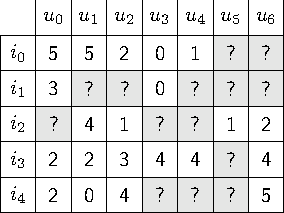
\includegraphics[width=.45\textwidth]{Chapters/06_RecommendationSystems/24_collaborativefiltering/latex/utility.pdf}
    }
\end{figure}
% ******************************************************************************
 
Vậy mỗi dấu `?' nên được thay bởi giá trị nào để hạn chế sai lệch khi ước lượng? Lựa chọn đầu tiên có thể nghĩ đến là thay các dấu `?' bằng 0. Điều
này không thực sự tốt vì giá trị 0 dễ bị nhầm với với mức độ quan tâm thấp nhất; và
một người dùng chưa đánh giá một sản phẩm không có nghĩa là họ hoàn toàn không
quan tâm tới sản phẩm đó. Một giá trị {an toàn} hơn là trung bình cộng của khoảng giá trị, ở đây là 2.5 trên hệ thống đánh giá năm sao. Tuy nhiên, giá trị này có
nhược điểm đối với những người dùng {dễ tính} hoặc {khó tính}. Những 
người dùng dễ tính có thể đánh giá ba sao cho các sản phẩm họ không thích;
ngược lại, những người dùng khó tính có thể đánh giá ba sao cho
những sản phẩm họ thích. Việc thay đồng loạt các phần tử khuyết bởi 2.5 trong
trường hợp này chưa mang lại hiệu quả. 
% ****************************************************************************** 

Một giá trị khả dĩ hơn cho việc này là ước lượng các phần tử khuyết bởi giá
trị trung bình mà một người dùng đã đánh giá. Điều này giúp tránh việc một
người dùng quá khó tính hoặc dễ tính. Các giá trị ước lượng này phụ thuộc
vào từng
người dùng. Quan sát ví dụ trong Hình~\ref{fig:24_2}.

% \textbf{Chuẩn hoá dữ liệu} 
\index{hệ thống gợi ý -- recommendation system!ma trận tiện ích chuẩn hoá -- normalized utility matrix }
Hàng cuối cùng trong Hình \ref{fig:24_2}a là trung bình các đánh giá của mỗi
người dùng. Các giá trị cao tương ứng với những người dùng dễ tính và ngược lại. Khi đó, nếu tiếp tục trừ từ mỗi đánh giá đi giá trị trung bình này và thay các giá trị chưa biết bằng 0,
ta sẽ được một \textit{ma trận tiện ích chuẩn hoá}({normalized utility
matrix}) như trong Hình \ref{fig:24_2}b. Việc làm này có một vài ưu điểm:

\begin{itemize}
    \item Việc trừ mỗi giá trị đi trung bình cộng của {cột} tương ứng trong ma trận tiện ích khiến mỗi
    cột có cả những giá trị dương và âm. Những giá trị dương ứng với những sản phẩm được người dùng quan tâm hơn. Những ô có giá trị 0 tương ứng với việc người dùng chưa đánh giá sản phẩm tương ứng. Tâ cần đự đoán giá trị ở các ô này. 

    \item Về mặt kỹ thuật, số chiều của ma trận tiện ích là rất lớn với
    hàng triệu người dùng và sản phẩm, việc lưu toàn bộ các giá trị này
    trong một ma trận sẽ yêu cầu bộ nhớ lớn.
    Vì số lượng đánh giá biết trước thường là một số rất nhỏ so với kích thước
    của ma trận tiện ích, sẽ tốt hơn nếu chúng ta lưu ma trận này dưới dạng một
    ma trận thưa, tức chỉ lưu các giá trị khác không và vị trí của
    chúng. Vì vậy, tốt hơn hết, các dấu '?' nên được thay bằng giá trị '0', tức
    chưa xác định liệu người dùng có thích sản phẩm hay không. Việc này
    không những tối ưu bộ nhớ mà việc tính toán ma trận tương tự về sau hiệu quả hơn. Ở đây, phần tử ở hàng thứ $i$, cột thứ $j$ của ma
    trận tương tự là độ tương tự giữa người dùng thứ $i$
    và thứ $j$.
\end{itemize}
\index{tương tự cos -- consine similarity}
\index{hệ thống gợi ý -- recommendation system!ma trận tương tự -- similarity matrix}
Sau khi dữ liệu đã được chuẩn hoá, hàm tương tự thường được sử
dụng là \textit{tương tự cos} ({cosine similarity}):
\begin{equation} 
\text{cosine\_similarity}(\mathbf{u}_1, \mathbf{u}_2) =\text{cos}(\mathbf{u}_1, \mathbf{u}_2)  
=  \frac{\mathbf{u}_1^T\mathbf{u}_2}{ \|\mathbf{u}_1\|_2.\|\mathbf{u}_2\|_2}
\end{equation} 
Trong đó $\mathbf{u}_{1, 2}$ là các vector tương ứng với hai người dùng trong ma
trận tiện ích chuẩn hoá. Có một hàm trong Python giúp cách tính hàm số này một
cách hiệu quả, chúng ta sẽ thấy trong phần lập trình.
 
 \begin{figure}[t]
\centering
    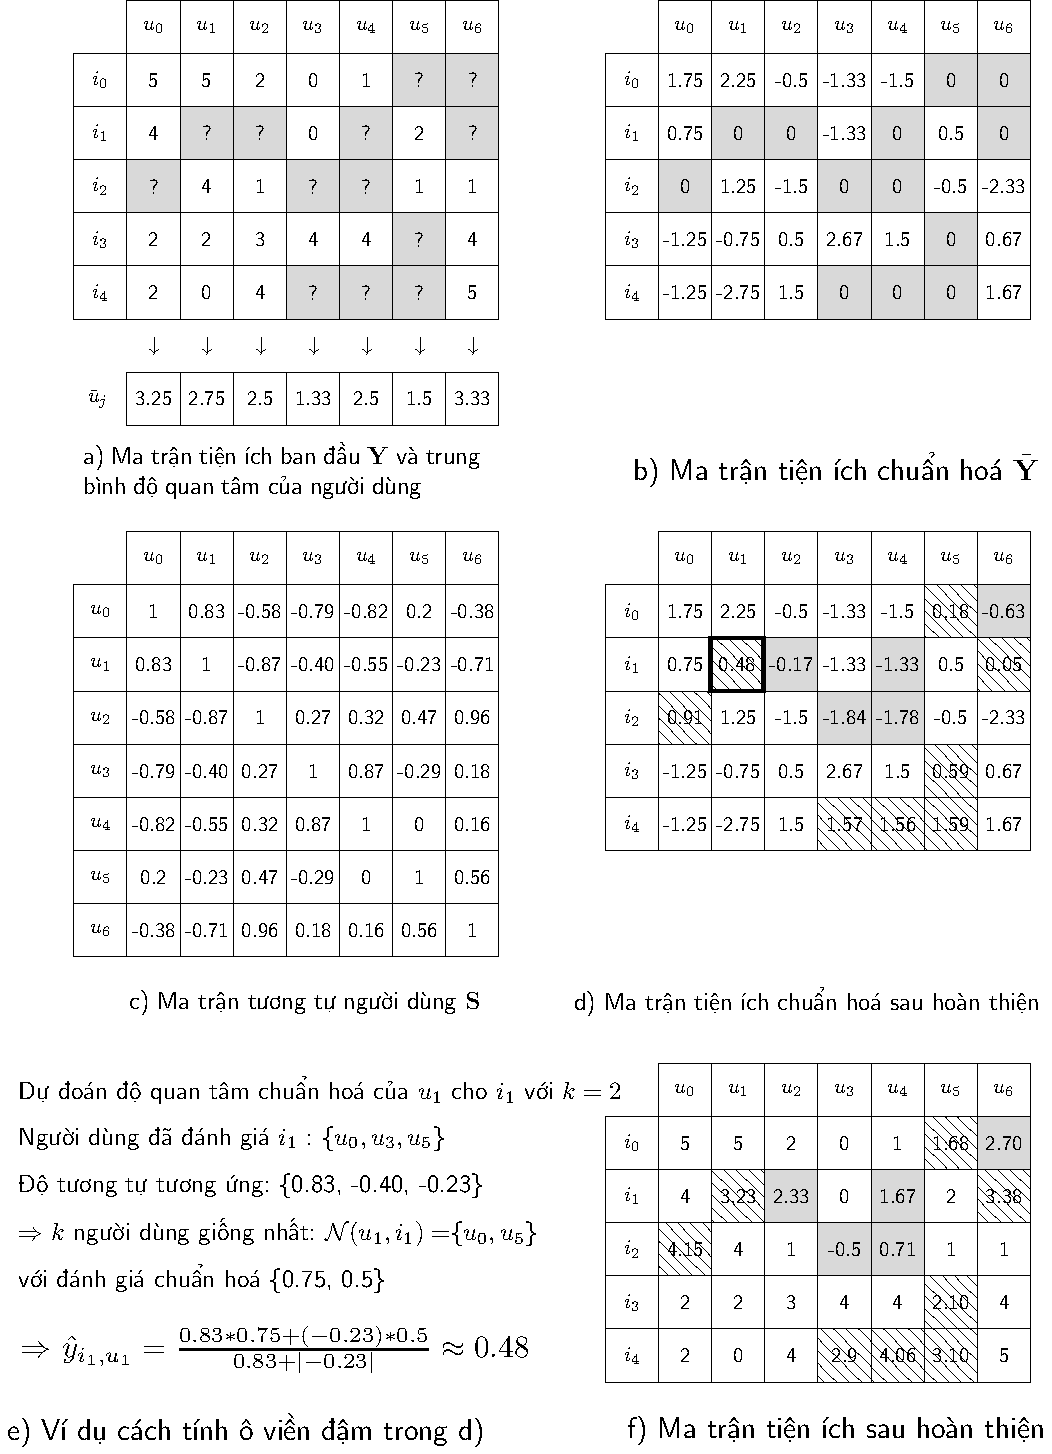
\includegraphics[width = .85\textwidth]{Chapters/06_RecommendationSystems/24_collaborativefiltering/latex/user_cf_gray_v.pdf}
    % 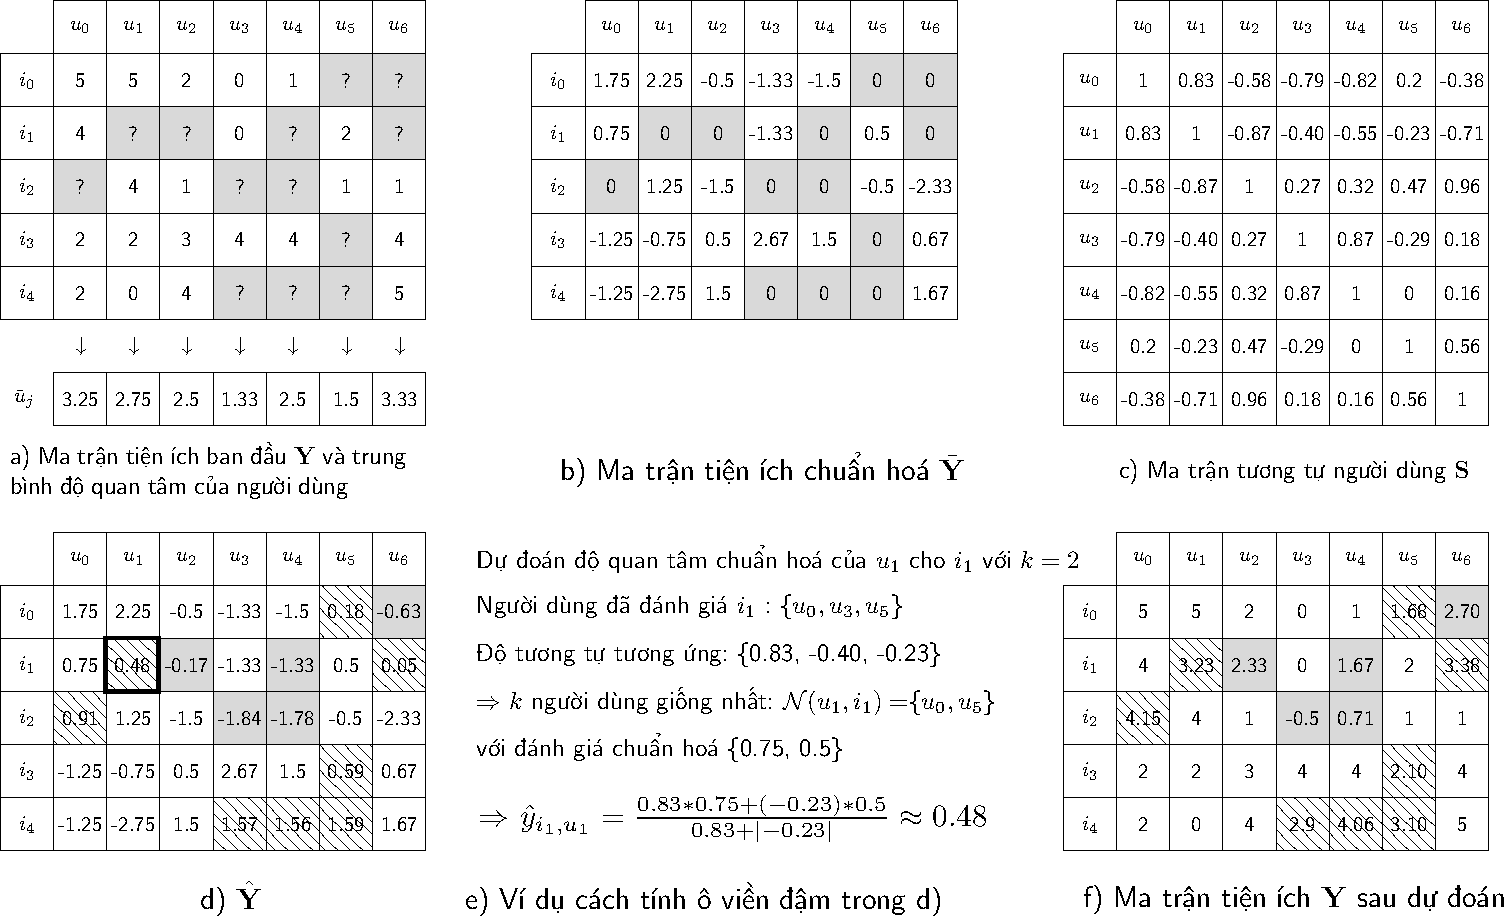
\includegraphics[width = \textwidth]{Chapters/06_RecommendationSystems/24_collaborativefiltering/latex/user_cf_gray.pdf}
    % 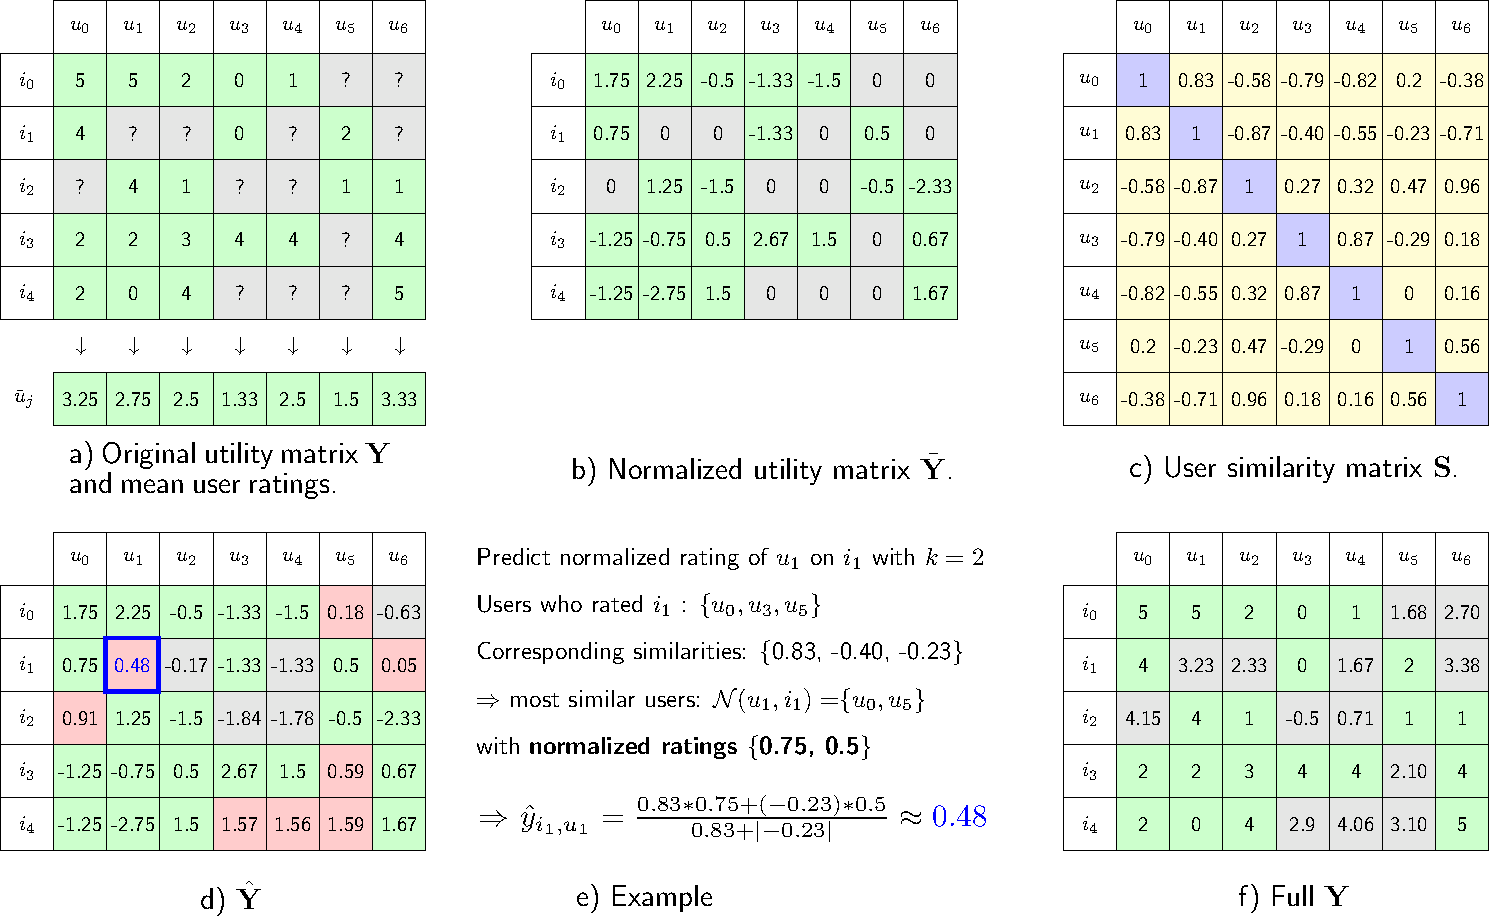
\includegraphics[width = \textwidth]{Chapters/06_RecommendationSystems/24_collaborativefiltering/latex/user_cf.pdf}
    \caption[]{Ví dụ mô tả lọc cộng tác người dùng. a) Ma trận tiện ích ban đầu. b) Ma trận tiện ích đã được chuẩn hoá. c) Ma trận tương tự giữa người dùng. d) Dự đoán độ quan tâm (chuẩn hoá) còn thiếu. e) Ví dụ về cách dự đoán độ quan tâm chuẩn hoá của $u_1$ tới $i_1$. f) Dự đoán các độ quan tâm còn thiếu.}
    \label{fig:24_2}
\end{figure}
% ****************************************************************************** 

Mức độ tương tự của hai vector là một số thực trong đoạn [-1, 1]. Giá
trị bằng 1 thể hiện hai vector hoàn toàn giống nhau. Hàm số
${\cos}$ của một góc bằng 1 xảy ra khi góc giữa hai vector bằng 0, tức hai
vector có cùng phương và cùng hướng. Giá trị của hàm ${cos}$ bằng -1 khi hai 
vector hoàn toàn trái ngược nhau, tức cùng phương nhưng khác hướng. Điều này có
nghĩa là nếu {hành vi} của hai người dùng là hoàn toàn
ngược nhau thì độ tương tự giữa họ là thấp nhất.
 
Ví dụ về tương tự cos của người dùng (đã được chuẩn
hoá) trong Hình~\ref{fig:24_2}b được cho trong Hình~\ref{fig:24_2}c.
Ma trận tương tự $\mathbf{S}$ là
một ma trận đối xứng vì $\cos$ là một hàm chẵn\footnote{Một hàm số
$f:\R\rightarrow \R$ được gọi là \textit{chẵn} nếu $f(x) = f(-x),~\forall x \in
\R$.}, và nếu $A$ tương tự $B$ thì điều
ngược lại cũng đúng. Các ô trên đường chéo đều là
$\text{cos}$ của góc giữa một vector và chính nó, tức $\text{cos}(0) = 1$. Khi
tính toán ở các bước sau, chúng ta không cần quan tâm tới các giá trị này.
Tiếp tục quan sát các vector hàng tương ứng với $u_0, u_1, u_2$, chúng ta sẽ
thấy một vài điều thú vị:

\begin{itemize}
    \item $u_0$ {gần} với $u_1$ và $u_5$ (độ tương tự là dương) hơn các
    người dùng còn lại. Việc độ tương tự cao giữa $u_0$ và $u_1$ là
    dễ hiểu vì cả hai đều có xu hướng quan tâm tới $i_0, i_1, i_2$ hơn các
    sản phẩm còn lại. Việc $u_0$ \textit{gần} với $u_5$ thoạt đầu có vẻ vô
    lý vì $u_5$ đánh giá thấp các sản phẩm mà $u_0$ đánh giá cao
    (Hình~\ref{fig:24_2}a); tuy nhiên khi nhìn vào ma trận tiện ích đã chuẩn hoá
    trong Hình~\ref{fig:24_2}b, ta thấy rằng điều này là hợp lý vì sản phẩm duy
    nhất mà cả hai người dùng này đã cung cấp thông tin là $i_1$ với các giá
    trị tương ứng đều lớn hơn không, tức đều mang hướng tích cực.
     
    \item $u_1$ gần với $u_0$ và xa những người dùng còn lại.  
     
\item $u_2$ gần với $u_3, u_4, u_5, u_6$ và xa những người dùng còn lại.  
\end{itemize}
 
Từ ma trận tương tự này, ta có thể phân các người dùng ra thành hai cụm $\{u_0,
u_1\}$ và $\{u_2, u_3, u_4, u_5, u_6\}$. Vì ma trận $\mathbf{S}$ nhỏ nên chúng ta
có thể quan sát thấy điều này; khi số người dùng lớn hơn, việc xác định bằng mắt
thường là không khả thi. Thuật toán \textit{phân cụm người dùng} ({users
clustering}) sẽ được trình bày trong chương tiếp theo.
 
% Một lưu ý nhỏ ở đây là khi số lượng người dùng lớn, ma trận
% $\mathbf{S}$ sẽ yêu cầu nhiều bộ nhớ hơn để lưu trữ. Với các
% trường hợp đó, chúng ta chỉ cần tính và lưu kết quả của
% một hàng của ma trận tương tự tương ứng với người dùng đó. 
 
% Trong bài viết này, tôi sẽ sử dụng \textit{similarity function} này.  
 
% \textbf{Person corelation:}  
 
% Tôi xin không đi chi tiết về phần này, bạn đọc quan tâm có thể đọc thêm \href{https://en.wikipedia.org/wiki/Pearson_correlation_coefficient}{Pearson correlation coefficient - Wikipedia} 
 
 
\subsection{Hoàn thiện ma trận tiện ích}
 
Việc {dự đoán mức độ quan tâm} của một
người dùng tới một sản phẩm dựa trên các người dùng tương tự này khá giống với 
{K lân cận} (KNN) với hàm khoảng cách được thay bằng hàm tương tự. 
 
Giống với như KNN, NBCF cũng dùng thông tin của $k$ người dùng lân cận để dự
đoán. Tất nhiên, để đánh giá độ quan tâm của một người dùng lên một
sản phẩm, chúng ta chỉ quan tâm tới những người dùng
đã đánh giá sản phẩm đó trong lân cận. {Giá trị cần điền} thường được xác
định là {trung bình có trọng số} của các đánh giá đã chuẩn hoá. Có một điểm cần lưu ý, trong KNN, các trọng số được xác định dựa trên
khoảng cách giữa hai điểm, và các khoảng cách này luôn là các số không âm.
Trong NBCF, các trọng số được xác định dựa trên độ tương tự giữa hai
người dùng. Những trọng số này có thể là các số âm. Công thức phổ biến được sử
dụng để dự đoán độ quan tâm của người dùng $u$ tới sảm phẩm $i$
là:\footnote{Sự khác biệt so với trung bình có trọng số là mẫu số có sử dụng trị
tuyệt đối.}
\begin{equation} 
\hat{y}_{i, u} = \frac{\sum_{u_j \in \mathcal{N}(u, i)} \bar{y}_{i, u_j} \text{sim}(u, u_j)}{\sum_{u_j \in \mathcal{N}(u, i)} |\text{sim}(u, u_j)|}
\end{equation} 
trong đó $\mathcal{N}(u, i)$ là tập hợp $k$ người dùng tương tự với $u$ nhất \textit{đã đánh giá} $i$.
Hình~\ref{fig:24_2}d hoàn thiện
ma trận tiện ích đã chuẩn hoá. Các ô
nền sọc chéo thể hiện các giá trị dương, tức các sản phẩm nên được gợi ý tới người dùng tương ứng. Ở đây, ngưỡng được lấy là 0, ngưỡng này
hoàn toàn có thể được thay đổi tuỳ thuộc vào việc ta muốn gợi ý nhiều hay ít
sản phẩm. 

Một ví dụ về việc tính độ quan tâm chuẩn hoá của $u_1$ tới $i_1$ được cho
trong Hình~\ref{fig:24_2}e với số lân cận $k = 2$. Các
bước thực hiện như sau:
\begin{enumerate}
    \item Xác định những người dùng đã đánh giá $i_1$, ở đây là $u_0, u_3,
    u_5$.
     
    \item  Mức độ tương tự giữa $u_1$ và những người dùng
    này lần lượt là $\{0.83, -0.40, -0.23\}$. Hai ($k = 2$) giá trị lớn nhất là
    $0.83$ và $-0.23$ tương ứng với $u_0$ và $u_5$.
     
    \item Xác định các đánh giá (đã chuẩn hoá) của $u_0$ và $u_5$ tới $i_1$, ta
    thu được hai giá trị lần lượt là $0.75$ và $0.5$.
     
    \item Dự đoán kết quả:
    \begin{equation} 
        \hat{y}_{i_1, u_1} = \frac{0.83\times 0.75 + (-0.23)\times 0.5}{0.83 + |-0.23|} \approx 0.48 
    \end{equation} 
\end{enumerate}
 
Việc quy đổi các giá trị đánh giá chuẩn hoá về thang năm có thể được thực hiện
bằng cách cộng các cột của ma trận $\hat{\mathbf{Y}}$ với giá trị
đánh giá trung bình của mỗi người dùng như đã tính trong
Hình~\ref{fig:24_2}a. Việc hệ thống quyết định gợi ý sản phẩm nào cho mỗi
người dùng có thể được xác định bằng nhiều cách khác nhau. Hệ thống có thể
sắp xếp các sản phẩm chưa được đánh giá theo độ giảm dần của mức độ quan tâm được dự đoán, hoặc có thể chỉ chọn các sản phẩm có độ quan tâm chuẩn hoá dương -- tương ứng với việc người dùng
này có nhiều khả năng thích hơn.
 
 
% Trước khi vào phần lập trình cho User-user CF, chúng ta cùng xem xét Item-item CF.  
 
\section{Lọc cộng tác sản phẩm}
\label{sec:ii}
\index{hệ thống gợi ý -- recommendation system!lọc cộng tác sản phẩm -- item-item collaborative filtering}
Lọc cộng tác người dùng có một số hạn chế như sau: 
\begin{itemize}
    \item Khi lượng người dùng lớn hơn số lượng sản phẩm (điều này thường xảy ra), mỗi chiều của ma trận tương tự bằng với số lượng người dùng. Việc lưu trữ một ma
    trận với kích thước lớn đôi khi không khả thi. 

    \item Ma trận tiện ích $\mathbf{Y}$ thường rất thưa, tức chỉ có
    một tỉ lệ nhỏ các phần tử đã biết. Khi lượng người dùng lớn so với lượng sản phẩm, nhiều cột của ma trận này có ít phần tử khác không vì người dùng thường \textit{lười} đánh giá
    sản phẩm. Vì thế, khi một người dùng thay đổi hoặc thêm các đánh giá, trung bình
    cộng các
    đánh giá cũng như vector chuẩn hoá tương ứng với người dùng này
    thay đổi theo. Kéo theo đó, việc tính toán ma trận tương tự, vốn tốn
    nhiều bộ nhớ và thời gian, cần được thực hiện lại. 
\end{itemize}

Có một cách tiếp cận khác, thay vì tìm sự tương tự giữa các người dùng, ta
có thể tìm sự tương tự giữa các sản phẩm. Từ đó nếu một người dùng
thích một sản phẩm thì hệ thống nên gợi ý các sản phẩm tương tự tới
người dùng đó. 

Khi lượng sản phẩm nhỏ hơn lượng người dùng, việc xây dựng mô hình dựa trên dự tương tự giữa các sản phẩm có một số ưu điểm:
\begin{itemize}
    \item Ma trận tương tự (vuông) có kích thước nhỏ hơn với số hàng bằng số sản phẩm. Việc này khiến việc lưu trữ và
    tính toán ở các bước sau được thực hiện một cách hiệu quả hơn. 


    \item Khi ma trận tiện ích có số hàng ít hơn số cột, trung bình số lượng phần tử đã
    biết trong mỗi hàng sẽ nhiều hơn trung bình số lượng phần tử đã biết trong
    mỗi cột. Nói cách khác, trung bình số sản phẩm được đánh giá bởi một người
    dùng sẽ ít hơn trung bình số người dùng đã đánh giá một sản phẩm. Kéo theo
    đó, việc tính độ
    tương tự giữa các hàng trong ma trận tiện ích cũng đáng tin cậy hơn. Hơn nữa, giá trị trung bình
    của mỗi hàng cũng thay đổi ít hơn khi có thêm một vài đánh giá. Như vậy,
    ma trận tương tự cần được cập nhật ít thường xuyên hơn.
\end{itemize}
 
Cách tiếp cận thứ hai này được gọi là \textit{lọc cộng tác sản phẩm} ({item-item CF}). Khi lượng sản phẩm ít hơn số lượng người dùng, phương
pháp này được ưu tiên sử dụng hơn.
 
Quy trình hoàn thiện ma trận tiện tích tương tự như trong lọc cộng tác người dùng, chỉ khác là bây giờ ta cần tính độ tương tự giữa các hàng của ma trận đó. 
\newnote{Liên hệ giữa lọc cộng tác sản phẩm và lọc cộng tác người dùng}{
    Về mặt toán học, lọc cộng tác sản phẩm có thể nhận được từ lọc cộng tác ngừoi dùng bằng cách
chuyển vị ma trận tiện ích và coi như sản phẩm đang đánh giá ngược người dùng. Sau khi hoàn thiện ma trận, ta cần chuyển vị một lần
nữa để thu được kết quả. }

% Từ khía cạnh lập trình, ta chỉ cần áp dụng thuật toán user-user CF lên ma trận utility chuyển vị của ma trận utility ban đầu.
% ******************************************************************************
\begin{figure}[t]
\centering
    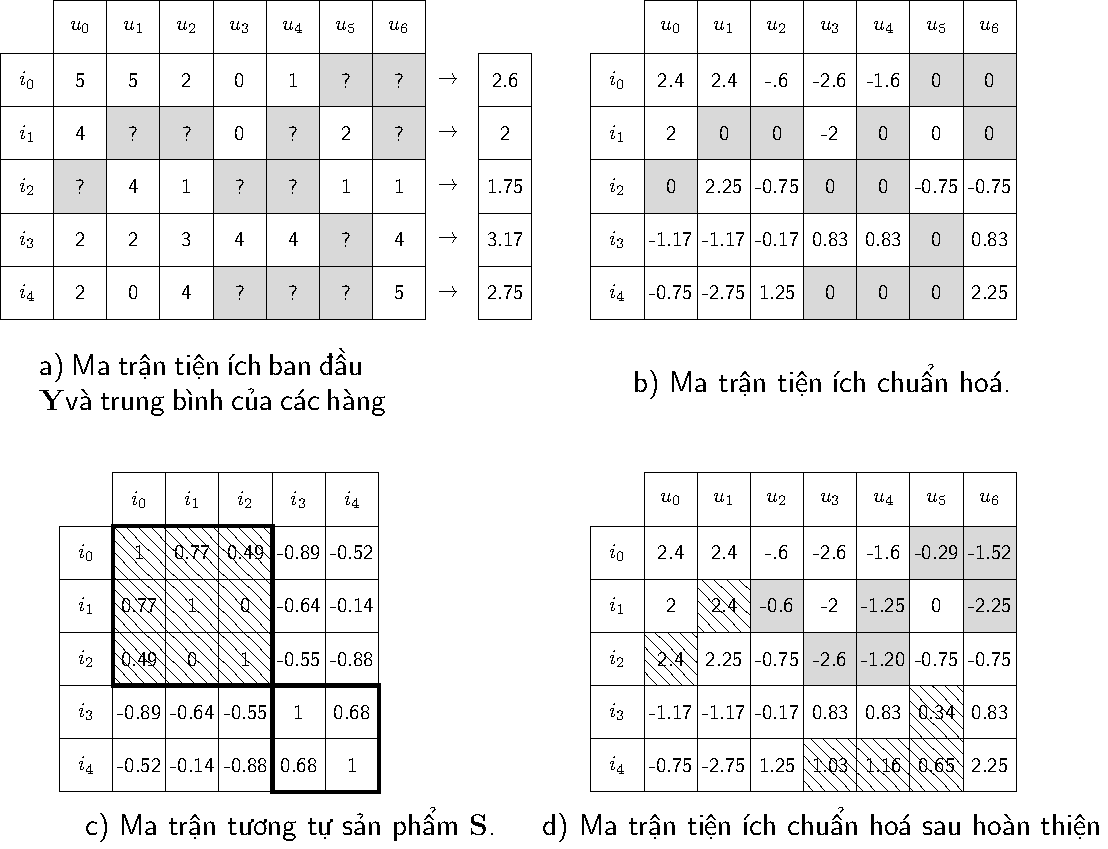
\includegraphics[width = \textwidth]{Chapters/06_RecommendationSystems/24_collaborativefiltering/latex/item_cf_gray.pdf}
    % 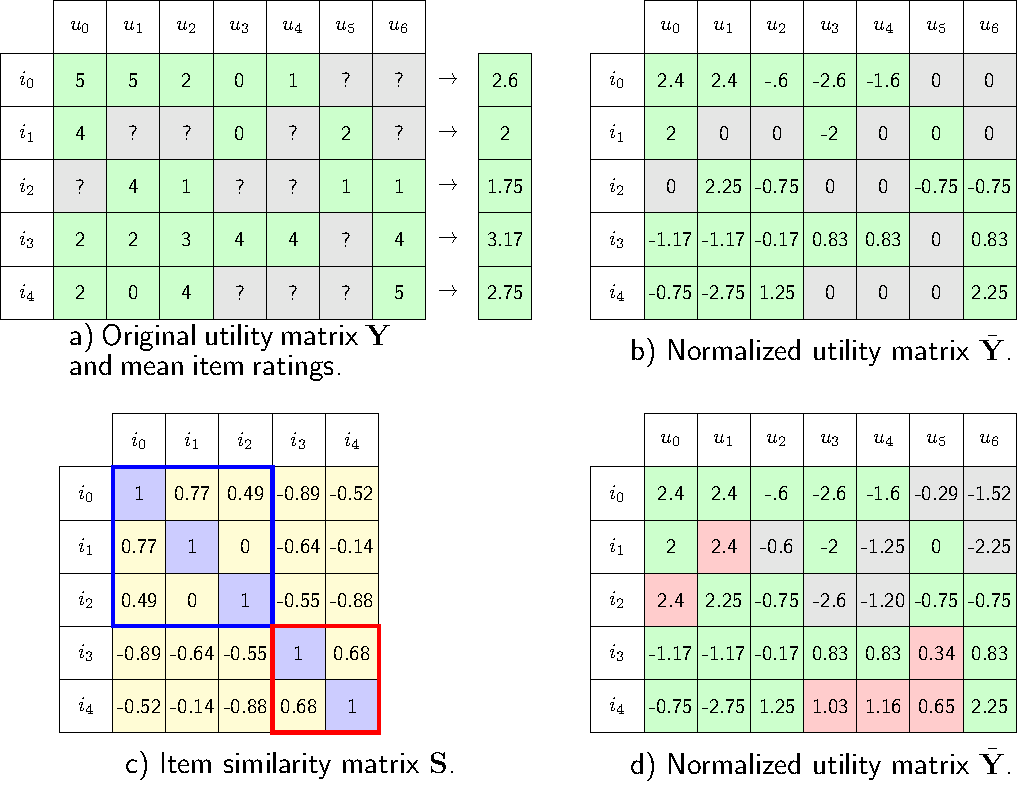
\includegraphics[width = \textwidth]{Chapters/06_RecommendationSystems/24_collaborativefiltering/latex/item_cf.pdf}
    \caption[]{Ví dụ mô tả item-item CF. a) Ma trận utility
    ban đầu. b) Ma trận utility  đã được chuẩn hoá. c) User similarity matrix.
    d) Dự đoán các (normalized) \textit{rating} còn thiếu.}
    \label{fig:24_3}
\end{figure}
% ******************************************************************************
 
Hình \ref{fig:24_3} mô tả quy trình này cho cùng ví dụ trong Hình~\ref{fig:24_2}. Một điểm
thú vị trong ma trận tương tự trong Hình \ref{fig:24_3}c là các phần tử trong
hai khu vực hình vuông lớn đều không âm, các phần tử bên ngoài
là các số âm. Việc này thể hiện rằng các sản phẩm có thể được chia thành
hai cụm rõ rệt. Như vậy, một cách {vô tình}, chúng ta đã thực
hiện việc phâm cụm sản phẩm. Việc này giúp ích cho việc dự
đoán ở phần sau vì các sản phẩm gần giống nhau rất có thể đã được phân vào
một cụm.
 Kết quả cuối cùng về việc chọn sản phẩm nào để gợi ý cho mỗi
người dùng được thể hiện bởi các ô có nền sọc chéo trong Hình \ref{fig:24_3}d. Kết quả
này có khác một chút so với kết quả tìm được bởi lọc cộng tác người dùng ở hai cột cuối
cùng tương ứng với $u_5, u_6$. Nhưng dường như kết quả này {hợp lý} hơn vì từ ma trận tiện ích, ta nhận thấy có hai nhóm người dùng có sở thích khác nhau. Nhóm thứ nhất là $u_0$ và $u_1$; nhóm thứ hai là những người dùng còn lại.
 
Mục~\ref{sec:24_python} sau đây mô tả cách lập trình cho NNCF trên
Python. Thư viện \pythoninline{sklearn} hiện chưa hỗ trợ các thuật toán gợi ý. Bạn đọc có thể tham khảo một thư viện khác khá tốt trên python là \pythoninline{surprise} (\url{http://surpriselib.com/}).
 
\section{Lập trình trên Python }
\label{sec:24_python}
Thuật toán lọc cộng tác tương đối đơn giản và không
chứa bài toán tối ưu nào. Chúng ta tiếp tục sử dụng bộ cơ sở dữ liệu MovieLens
100k như trong chương trước. \pythoninline{Class
uuCF} trong đoạn code dưới đây thực hiện quy trình lọc cộng tác người dùng. Có hai phương thức chính của
\pythoninline{class} này là \pythoninline{fit} -- tính ma trận tương tự, và
\pythoninline{predict} -- dự đoán số sao mà một người dùng sẽ đánh giá một
sản phẩm:
 \newpage 
\begin{lstlisting}[language=Python]
from __future__ import print_function 
import pandas as pd 
import numpy as np
from sklearn.metrics.pairwise import cosine_similarity
from scipy import sparse 

class uuCF(object):
    def __init__(self, Y_data, k, sim_func = cosine_similarity):
        self.Y_data = Y_data # a 2d array of shape (n_users, 3)
            # each row of Y_data has form [user_id, item_id, rating]
        self.k         = k # number of neighborhood
        # similarity function, default: cosine_similarity
        self.sim_func  = sim_func 
        self.Ybar      = None   # normalize data 
        # number of users
        self.n_users   = int(np.max(self.Y_data[:, 0])) + 1 
        # number of items
        self.n_items   = int(np.max(self.Y_data[:, 1])) + 1
    
    def fit(self):
        # normalized Y_data -> Ybar 
        users = self.Y_data[:, 0] # all users - first column of Y_data
        self.Ybar = self.Y_data.copy()
        self.mu = np.zeros((self.n_users,))
        for n in xrange(self.n_users):
            # row indices of ratings made by user n
            ids      = np.where(users == n)[0].astype(np.int32)
            # indices of all items rated by user n 
            item_ids = self.Y_data[ids, 1] 
            # ratings made by user n 
            ratings  = self.Y_data[ids, 2]  
            # avoid zero division 
            self.mu[n] = np.mean(ratings) if ids.size > 0 else 0 
            self.Ybar[ids, 2] = ratings - self.mu[n]
            
        # form the rating matrix as a sparse matrix. 
        # see more: https://goo.gl/i2mmT2
        self.Ybar = sparse.coo_matrix((self.Ybar[:, 2],
            (self.Ybar[:, 1], self.Ybar[:, 0])), 
            (self.n_items, self.n_users)).tocsr()
        self.S = self.sim_func(self.Ybar.T, self.Ybar.T)
    
    def pred(self, u, i):
        """ predict the rating of user u for item i"""
        # find item i 
        ids = np.where(self.Y_data[:, 1] == i)[0].astype(np.int32) 
        # all users who rated i
        users_rated_i = (self.Y_data[ids, 0]).astype(np.int32) 
        sim = self.S[u, users_rated_i]  # sim. of u and those users
        
        nns = np.argsort(sim)[-self.k:] # most k similar users 
        nearest_s = sim[nns] # and the corresponding similarities        
        r   = self.Ybar[i, users_rated_i[nns]] # the corresponding ratings 
        eps = 1e-8 # a small number to avoid zero division 
        return (r*nearest_s).sum()/(np.abs(nearest_s).sum()+eps)+self.mu[u]
    
\end{lstlisting}

Tiếp theo, ta áp dụng vào MoviesLen 100k:
\begin{lstlisting}[language=Python]
r_cols = ['user_id', 'movie_id', 'rating', 'unix_timestamp']
ratings_base = pd.read_csv('ml-100k/ua.base', sep='\t', names=r_cols)
ratings_test = pd.read_csv('ml-100k/ua.test', sep='\t', names=r_cols)
rate_train = ratings_base.as_matrix()
rate_test = ratings_test.as_matrix()
rate_train[:, :2] -= 1 # since indices start from 0
rate_test[:, :2] -= 1
rs = uuCF(rate_train, k = 40)
rs.fit()
n_tests = rate_test.shape[0]
SE = 0 # squared error
for n in xrange(n_tests):
    pred = rs.pred(rate_test[n, 0], rate_test[n, 1])
    SE += (pred - rate_test[n, 2])**2 

RMSE = np.sqrt(SE/n_tests)
print('User-user CF, RMSE =', RMSE)
\end{lstlisting}
\kq
\begin{lstlisting}[language=Python]
User-user CF, RMSE = 0.976614028929
\end{lstlisting}

Như vậy, trung bình mỗi đánh giá bị dự đoán lệch khoảng 0.976. Kết quả này tốt hơn kết quả có được bởi gợi ý dựa trên nội dung trong chương trước. 

Tiếp theo, chúng ta áp dụng lọc cộng tác sản phẩm vào tập cơ sở dữ
liệu này. Để áp dụng lọc cộng tác sản phẩm, ta chỉ cần chuyển vị ma trận tiện ích. Trong trường hợp này, vì ma trận tiện ích được lưu dưới dạng
\pythoninline{[user_id, item_id, rating]} nên ta chỉ cần đổi chỗ cột thứ nhất
cho cột thứ hai của \pythoninline{Y_data}:

\begin{lstlisting}[language=Python]
rate_train = rate_train[:, [1, 0, 2]]
rate_test  = rate_test[:, [1, 0, 2]]

rs = uuCF(rate_train, k = 40)
rs.fit()

n_tests = rate_test.shape[0]
SE = 0 # squared error
for n in xrange(n_tests):
    pred = rs.pred(rate_test[n, 0], rate_test[n, 1])
    SE += (pred - rate_test[n, 2])**2 

RMSE = np.sqrt(SE/n_tests)
print('Item-item CF, RMSE =', RMSE)
\end{lstlisting}
\kq 
\begin{lstlisting}[language=Python]
Item-item CF, RMSE = 0.968846083868
\end{lstlisting}
Như vậy, trong trường hợp này lọc cộng tác sản phẩm cho kết quả tốt
hơn, ngay cả khi số sản phẩm (1682) lớn hơn số người dùng (943).
Với các bài toán khác, chúng ta nên thử cả hai phương pháp trên một tập xác thực và chọn
ra phương pháp cho kết quả tốt hơn. Kích thước lân cận $k$ cũng có thể được thay bằng các giá trị khác. 
 
 
\section{Thảo luận}
\label{sec:24_discuss}
\begin{itemize}
    \item Lọc cộng tác là một phương pháp gợi ý sản phẩm dựa trên hành vi của các người dùng tương tự khác lên cùng một
    sản phẩm. Việc làm này được thực hiện dựa trên sự tương tự giữa người dùng được mô tả bởi ma trận tương tự.
 
    \item Để tính ma trận tương tự, trước tiên ta cần chuẩn hoá dữ
    liệu. Phương pháp chuẩn hoá dữ liệu phổ biến là trừ mỗi cột (hoặc hàng) của ma trận tiện ích đi trung bình của các phần tử đã biết trong cột (hàng) đó. 
 
    \item Hàm tương tự thường dùng là tương tự cos. 
 
    \item Một hướng tiếp cận khác là thay vì đi tìm các người dùng tương tự với một người dùng (lọc cộng tác người dùng), ta đi tìm các sản phẩm tương tự
    với một sản phẩm cho trước (lọc cộng tác sản phẩm). Trong nhiều trường hợp, lọc cộng tác sản phẩm mang lại kết quả tốt hơn. 


    \item Mã nguồn trong chương này có thể được tìm thấy tại \url{https://goo.gl/vGKjbo}.
\end{itemize}
 
 
\subsubsection{Đọc thêm}
\begin{enumerate}
    \item[1.] M. Ekstrand \etal, \textit{Collaborative filtering recommender systems.}
    (\url{https://goo.gl/GVn8av}) Foundations and Trends® in Human–Computer Interaction 4.2 (2011): 81-173.
\end{enumerate} 
 
